%\section{Co-construction et accompagnement, un état de l'art}
%\subsection{Modéliser des dynamiques spatiales en contexte interdisciplinaire}
%\subsection{Le cas du \textit{companion modelling}}
%\subsection{L'exploration interactive comme interface disciplinaire}
%
%\section{Un retour sur une expérience de co-construction de modèle}
%\subsection{Cadre de l'expérience : groupe de travail et temporalités}
%\subsection{Conditions de l'expérience : quelle modélisation ?}
%\subsection{Déroulement de l'expérience}
%
%\section{Une méthode de co-construction faite d'allers-retours interdisciplinaires}
%\subsection{Un langage et des outils communs : préférer la co-construction à la prestation}
%\subsection{Modéliser pour explorer, explorer pour modéliser : comment combiner et accumuler les connaissances acquises}
%\subsection{Du particulier au générique : médiation et compromis entre disciplines}
%
%\section{Modéliser en géographe}
%\subsection{Observer un territoire passé : l'impossible terrain}
%\subsection{Modèle spatiaux et modèles spatialisés}
%\subsection{Modéliser en géographe, ne pas modéliser pour les géographes}

\chapter{Modélisation et visualisation comme interfaces disciplinaires}
\label{chap:chap1}
\begin{center}
	{\large Version \hl{2019-10-16}}
\end{center}

\begin{itemize}
	\item 10/10/2019 : Nouveau plan
	\item 14/10/2019 : fin 1.1
	\item 16/10/2019 : fin 1.2
\end{itemize} 

\minitoc

\clearpage
\section*{Introduction}
\addcontentsline{toc}{section}{\protect\numberline{}Introduction}

\begin{itemize}
	\item faire parallèles entre modélisation et juridique etc. : on connait le modèle, on l'a créé, et on connait le fonctionnement précis de ses composantes. Mais pas possible de deviner tous les biais que cela engendre de manière interne (bugs, == détournements de loi), et surtout les effets généraux causés par les interactions (politique sociale contre effet par exemple) ==> On a construit le modèle, mais on ne peut en prévoir l'aboutissement.
	\item Parler de l'approche exploratoire : explo de données vs explo de modèle, Ana Sensib vs CAH etc. chap  6
	\item Parler des connaissances expertes : pas de source, manque de connaissance de l'historiographie, donc on fait confiance aux notes et mémoire.
	\item 
\end{itemize}


\section{D'où je viens}

Le travail de recherche présenté dans cette thèse s'inscrit profondément à l'interface entre plusieurs courants disciplinaires liés à l'étude des phénomènes sociaux dans l'espace.
Pour en comprendre aussi bien le questionnement que l'approche mobilisée et les résultats obtenus, il me\footnote{
	Dans ce chapitre, très personnel et consacré essentiellement à la description et justification d'un positionnement individuel, le choix de la première personne du singulier me semble tout à fait adapté.
	Dans le reste de ce manuscrit, qui relate une expérience collective, la première personne du pluriel sera exclusivement mobilisée.
} paraît important de faire un rapide retour sur ma formation initiale et début de parcours dans le monde de la recherche académique, qui explique et préfigure assez largement le positionnement adopté dans ce travail.
Depuis une formation classique de géographie humaine et urbaine jusqu'à l'exercice de fonctions d'ingénieur d'étude en modélisation, en passant par une spécialisation en géomatique et cartographie, chacune des étapes de ma formation permet ainsi de mieux appréhender et comprendre l'aboutissement à cette thèse basée sur la co-construction interdisciplinaire de modèles spatiaux et sur leur exploration graphique.

\subsection{Géographie}

Ce travail de recherche s'inscrit avant tout, tant administrativement que conceptuellement, dans le champ disciplinaire de la géographie.
Cette discipline, consacrée à l'étude de la dimensions spatiale de phénomènes sociaux, constitue les fondements de ma formation initiale.
En sortant de classes préparatoires littéraires généralistes, j'avais ainsi été frappé par l'exercice du commentaire de cartes, à visée tant verticale (cartes géologiques) qu'horizontale (cartes topographiques), permettant de décrire et d'expliquer le fonctionnement humain d'un lieu par la seule observation de ses structures et contextes spatiaux.

\paragraph{Géographie urbaine.}
Cela m'a mené vers un cursus classique de géographie, majoritairement marqué par la géographie humaine et la recherche de grandes tendances spatiales dans les interactions sociales humaines.
Avec un intérêt pour l'aménagement et l'urbanisme, la géographie urbaine, dans sa dimension sociale, m'est rapidement apparue comme particulièrement stimulante, dans sa capacité à décrypter, à expliquer et à comparer des processus sociaux variés à l'échelle intra-urbaine.
Il ne s'agissait plus simplement de décrire un état, mais d'expliquer les processus spatiaux et sociaux y ayant mené.
Au regard des enseignements d'urbanisme et de politiques de la ville, ces approches permettaient ainsi de comparer le résultat de différentes politiques publiques, et de mener un début de mesure objective de l'écart entre leur objectif exprimé et leur action effective.

En master, j'ai voulu appliquer ces approches en initiant, sous la co-direction de Renaud Le Goix et Antonine Ribardière, un mémoire sur le thème de la comparaison de l'intégration spatiale des migrants entre les politiques francophones et anglophones.
Les politiques migratoires francophones, nourries du modèle jacobin français, menaient-elles à une plus forte inclusion et mixité sociale que les modèles anglophones, fondés sur l'image d'un \og \textit{salad-bowl}\fg{} communautaire ?
Le cas d'étude choisi portait sur le Canada, pays ayant l'avantage de présenter ces deux communautés linguistiques et culturelles, d'avoir une forte culture et attraction migratoire aussi bien pour les pays les plus développés que pour les Suds, et enfin de tenir un recensement permettant les études ethniques et communautaires.

\paragraph{Géographie Théorique et Quantitative.}
Dans un contexte de découverte de l'analyse spatiale, de la modélisation graphique, des systèmes d'information géographiques (SIG) et d'approches plus systémiques et horizontales de description et d'explication de phénomènes socio-spatiaux, ce travail s'est assez rapidement orienté vers une démarche quantitative et à visée plus généralisante.
Le mémoire qui en a résulté, intitulé \og Ségrégation spatiale et origines ethniques dans les métropoles canadiennes\fg{}, illustre ce tournant vers la géographie théorique et quantitative (GTQ) et cette volonté d'approche très quantifiée, en faisant la part belle à la comparaison des différents indices de ségrégation caractérisant les distributions spatiales de la population urbaine canadienne.
Pour être en mesure de mener cette comparaison systématique, une auto-formation poussée avait été nécessaire, notamment sur les techniques d'analyse de données, de réduction de dimensionalité (les recensements canadiens contiennent des centaines de catégorie qui ne pouvaient toutes êtres traitées individuellement) et sur une première approche d'automatisation de traitements (via SAS) pour être en mesure de tester rapidement différentes hypothèses sur les quelques milliers de \og secteurs de recensement\fg{} impliqués dans l'étude.

Du point de vue méthodologique, cette première expérience d'exploration systématique d'un jeu de données hétérogène et qu'il fallait caractériser par le calcul d'une dizaines d'indices de ségrégation, globaux et locaux, m'avait montré la nécessité de parvenir à une certaine automatisation de la chaîne de traitement, depuis la sélection des données, le calcul de tel ou tel indice, jusqu'à leur représentation (carto)graphique.
Les quelques macros SAS mises en place ne permettaient alors pas une automatisation totale de cette démarche d'analyse, et les mois d'été passés aux traitements systématiques et répétitifs nécessaires à une approche comparative ne rendaient que plus criant le besoin d'une méthode intégrée et automatisée.

\subsection{Géomatique}

C'est donc à la recherche de ces éléments que je me suis orienté, pour le master 2, vers une spécialisation en géomatique et cartographie, en intégrant le master professionnel Carthagéo.
Les connaissances, méthodologiques et techniques, que j'y ai acquis sont importantes et ont toutes concouru aux démarches mises en place dans ce travail de thèse.

\paragraph{Programmation, automatisation et interfaces graphiques.}
En premier lieu, Carthagéo m'a permis de découvrir des méthodes d'automatisation de chaînes de traitement de données spatiales.
Avec ces initiations à la programmation, une vision algorithmique, systématique et processuelle, devenait un pré-supposé obligatoire : pour automatiser un traitement, il fallait avant tout pouvoir le formaliser, sur papier d'abord, de manière à pouvoir en réaliser une implémentation informatique.
C'est, pour moi, la découverte de la mise en place de modèles graphiques, non plus dédiés à la description d'un lieu mais à l'explicitation d'un processus.
Avec l'automatisation permise par l'implémentation de ces chaînes de traitement, il devenait aussi possible de mener des études systématiques, reproductibles et paramétrées.

Dans le cadre d'un projet de programmation SIG, j'ai aussi du réaliser un outil, sous la forme d'un \textit{plugin}, permettant une comparaison visuelle et mesurée de la qualité de géocodage de différents services.
En dehors de l'aspect technique, cette première expérience de projet de programmation appliqué a surtout été l'occasion de réfléchir à des questions d'interface homme-machine.
Comment rendre intuitif, pour un évaluateur détaché du sujet, l'usage d'un outil interactif pensé pour vérifier la cohérence de géocodage de différentes adresses ? Fallait-il privilégier la présentation de l'indicateur quantitatif  -- la distance entre les points issus du géocodage -- ou plutôt donner une idée plus contextuelle de la localisation spécifique des résultats du géocodage ?
Paradoxalement, cet apprentissage de la programmation et de l'automatisation débouchait sur des questionnements relatifs au développement et à l'usage d'une interface graphique.
Cette sensibilité à l'\og usabilité\fg{} d'un logiciel a été très présente dans la suite, et me paraît fortement visible dans le présent travail de thèse (voir \hl{partie 5.4}).

\paragraph{Approches géométriques.}
Une autre approche extrêmement mobilisée dans cette thèse consiste dans une vision processuelle \og géométrique\fg{} des traitements de données spatiales.
Dans ce type d'approches, caractérisée par les recours aux opérateurs spatiaux, les agrégations, extractions et filtrages de données sont réalisés de manières surtout spatiales.
Il s'agit de prendre en compte le contexte spatial, topologique, pour réaliser les opérations sur les données.
En somme, cela revient à mobiliser la dimension spatiale des données dans les différentes chaînes de traitement mises en œuvre, et la différencier fortement des autres dimensions, attributaires.
Ces approches sont nécessaires à la réalisation d'analyses portant sur des données de différentes granularités, de différents maillages : elles permettent en effet d'homogénéiser des informations dont la dimension spatiale est primordiale.
En tant que telle, cette vision \og géométrique\fg{} nous a été fortement recommandée et transmise dans le cadre d'enseignements d'analyse spatiale.

Dans le modèle présenté dans cette thèse (\hl{chap2}), une large partie des mécanismes est caractérisé par des processus géométriques, qu'il s'agisse de la mise en place de zones tampons, de prises en compte du voisinage, de logiques de distances euclidiennes, d'intersections et unions spatiales etc.
L'influence de mon parcours me semble indéniable sur ces choix de modélisation où l'espace est traité de manière continue, assez peu répandus malgré tout dans les modèles de dynamiques spatiales.

\paragraph{Représentations (carto)graphiques.}
Un dernier point lié à mon enseignement de master a largement infusé sur les choix de ce travail de thèse.
Le master Carthagéo est une formation en grande partie dédiée à la cartographie, c'est-à-dire à l'apprentissage des \og règles\fg{} de représentation cartographiques et à une certaine réflexivité sur les différents messages qu'une carte peut convoyer.
La réflexion méthodologique sur les usages de la représentation (carto)graphique pour rendre compte d'un jeu de données est fortement présente dans l'ensemble des projets qui doivent être réalisés au cours de l'année de formation.
Les choix de représentation graphiques, très présents dans ce travail de thèse, ont ainsi durablement percolé depuis cet apprentissage.

\subsection{Modélisation : à la confluence de la GTQ et de la géomatique}

Master professionel oblige, la validation de Carthagéo impliquait la réalisation d'un stage de fin d'étude, en entreprise ou en unité de recherche.
J'ai eu la chance d'entamer un stage dans l'UMR Géographie-cités, en mai 2011, sous la co-direction de Thomas Louail, Clara Schmitt et Sébastien Rey-Coyrehourcq.
Ce stage, finalement intitulé \og Conception de modèles et d’outils de géosimulation \fg{} \autocite{cura_conception_2011}, était déjà organisé autour de tâches qui résonnent fortement vis-à-vis du contenu de la présente thèse.

Il s'agissait, de \og prendre part à toutes les étapes de la modélisation\fg{}, grâce à (1) l'enrichissement d'un modèle de simulation (SimpopLocal) ; (2) la participation à la conception et implémentation d'un second modèle de simulation (SimpopNet) ; (3) la création d'un outil de production de rapports de simulations (TrajPop) ; (4) la création d'un outil d'exploration cartographique des résultats de simulation \autocite[12-13]{cura_conception_2011}.
Ce stage de six mois, et les deux années de contrats d'ingénieur d'étude qui l'ont suivi et ont permis d'en prolonger les recherches (au sein des projets GeoDiverCity, MIRO² puis TransMonDyn)\footnote{
	Respectivement portés par Denise Pumain (ERC GeoDiverCity), Arnaud Banos (ANR MIRO²) et Lena Sanders (ANR TransMonDyn).
} ont durablement marqué mon rapport à la modélisation, à l'utilité de telles méthodes et à la manière de construire un modèle de façon collective.

\paragraph{Découverte de la modélisation à base d'agents.}
Ce stage a marqué ma découverte du domaine de la modélisation, et en particulier de la modélisation à base d'agents.
Coïncidentiellement, le premier modèle que j'ai eu à comprendre et à enrichir était un modèle de simulation de l'émergence et de la hiérarchisation d'un système de peuplement sur le temps long, au néolithique : SimpopLocal \autocite{schmitt_modelisation_2014,rey-coyrehourcq_plateforme_2015}.
Il s'agissait donc de tester des hypothèses issues de la géographie théorique et quantitative en les testant, \textit{in silico}, à l'aide d'un outil informatique permettant de simuler des dynamiques spatiales.

Pour que je parvienne à comprendre et à m'approprier le modèle, mes encadrants m'avaient demandé d'ajouter un mécanisme exogène de perturbation du système simulé, sous la forme d'incidences de catastrophes naturelles. 
L'idée de mon implication était de me permettre de me former, par la pratique, aux notions sous-jacentes de la modélisation de systèmes complexes : émergence, interactions entre agents, processus endogènes et exogènes etc.

Ces éléments ont été mis en pratique dans la participation à la conception et à l'implémentation d'un second modèle de simulation, \og SimpopNet-Réseaux\fg{}, \og modèle-jouet\fg{} servant de prototype pour le modèle SimpopNet développé plus tard \autocite{schmitt_modelisation_2014}.
Il s'agissait cette fois-ci de modéliser la co-évolution entre systèmes de villes et réseaux de communication, en simulant des potentiels d'interactions entre villes par l'intermédiaire de réseaux routiers formalisés par des graphes.

\paragraph{Visualisation et évaluation de modèle.}
Pour rendre compte de ces deux modèles -- SimpopLocal et SimpopNet --, il m'avait été demandé de développer des outils de visualisation et d'exploration de leurs comportements.
Les outils de visualisation intégrés à la plateforme de modélisation, NetLogo, n'étaient en effet pas suffisants pour rendre compte des différentes dynamiques produites par ces modèles.
Dans un premier temps, pour étudier l'effet des perturbations sur SimpopLocal, j'ai implémenté un type de représentation utilisé pour montrer l'évolution des rangs des villes d'un système, en m'appuyant sur les \og rank clocks\fg{} de \textcite{batty_rank_2006}.
Cette visualisation \textit{ad hoc} était très adaptée, mais ne permettait d'évaluer qu'une unique dimension (la stabilité des rangs) des processus modélisés.
De plus, il était nécessaire de re-générer manuellement ces graphiques à chaque nouvelle sortie du modèle.

C'est par le biais de la recherche d'automatisation et de proposition de plusieurs modes de représentation que j'ai été amené à découvrir le langage R et ses possibilités de création de rapports automatiquement produits à partir de jeux de données.
L'outil qui en a découlé, intitulé TrajPop (analyse des trajectoires de population), a été en premier lieu mobilisé sur les populations simulées de SimpopLocal.
Cela marquait ainsi un premier pas vers une évaluation systématique des sorties de simulation, permettant de plus d'archiver de manière systématisée les résultats de simulation.
Par la suite, TrajPop a été employé et amélioré pendant plusieurs années pour caractériser l'évolution des populations de systèmes de villes empiriques et non plus simulés (par exemple dans \textcite{pumain_multilevel_2015}).

\paragraph{Accompagnement à la modélisation.}
Un dernier aspect hérité de mes années de stagiaire/ingénieur d'étude à l'UMR Géographi-cités concerne un mode particulier de modélisation, pleinement inscrit dans le travail collectif.
Il s'agit d'une approche collective, collaborative voir accompagnatrice de la modélisation.
En effet, si les modèles SimpopLocal et SimpopNet étaient pilotés par des doctorants-modélisateurs, j'ai aussi participé à une expérience de modélisation commune où mon rôle, mi-modélisateur mi-accompagnateur, consistait à formaliser et implémenter des hypothèses sur la constitution de réseaux de collaboration scientifique.
Marie-Noëlle Comin, géographe qui avait réalisé une thèse empirique sur le sujet \autocite{comin_reseaux_2009}, cherchait ainsi à tester différents scénarios explicatifs aux regroupement de chercheurs dans le cadre de la constitution de consortiums en vue de candidature à des financements de projets scientifiques : par affinité et historique de collaboration, par importance bibliométrique, par capacité passée à remporter des financements etc.

Le modèle issu de cette co-construction, SearchNet, a été élaboré pendant près de deux ans, en requérant une forte perméabilité de ses concepteurs aux thématiques et usages de l'autre.
Par faute de temps consacré à sa finalisation, ce modèle n'a finalement jamais été achevé et mobilisé dans une publication scientifique.
Cette expérience, que l'on pourrait qualifier d'avortée, m'a pourtant permis de réaliser que pour mener à terme un projet de modélisation fortement collectif, il était nécessaire de disposer de beaucoup de temps, de motivation, et qu'une partie non négligeable de ces deux ressources rares devait être dédiée à l'accoutumance, des deux côtés, aux thématiques et méthodologies mobilisées dans un modèle.


\paragraph[Conclusion intermédiaire]{}
Ma formation académique et mes expériences passées de modélisation à base d'agent, entre géographie et géomatique, ont considérablement influencé la manière dont le présent travail de recherche a été abordé.
Ces éléments n'expliquent pas, seuls, l'ensemble des choix faits dans cette thèse, mais peut-être permettent-ils de mieux les comprendre, qui plus est au regard du contexte dans lequel cette thèse a été conçue et réalisée.

\section{Dans quel contexte s'inscrit ce travail ?}

Le sujet initial de cette thèse a été conçu alors que j'étais ingénieur d'étude en analyse de données et représentations cartographiques, sous l'encadrement de Lena Sanders, pour le projet ANR TransMonDyn\footnote{
Programme \og Blanc\fg{} de l'Agence Nationale de la Recherche (ANR), sous le code \mbox{ANR-10-BLAN-1805},  \href{http://www.transmondyn.parisgeo.cnrs.fr/}{www.transmondyn.parisgeo.cnrs.fr}
}.
Ce projet interdisciplinaire, officiellement mené entre 2011 et 2014, visait à \og modéliser les grandes transitions de l'évolution du peuplement dans l'Ancien et le Nouveau Monde: contraintes environnementales, interactions spatiales et innovations sociales dans la dynamique multi-échelles de systèmes complexes\fg{}.

C'est au sein de ce projet que s'est constitué le groupe de travail qui a donné lieu à SimFeodal, et c'est dans TransMonDyn que ce modèle, les hypothèses sur lesquelles il repose et les grandes lignes conceptuelles qui l'animent ont été conçu.
Il me paraît donc indispensable de préciser les cadres conceptuels et pratiques de ce projet, et en particulier ceux qui ont ébauché les grandes directions empruntées dans cette thèse.

\subsection{Modélisation de processus spatiaux}

L'entrée principale de TransMonDyn était résolument spatiale.
Le projet cherchait à identifier et à modéliser de grandes transformations dans les systèmes de peuplements.
En préalable au lancement du projet, la quarantaine de participants initiaux avaient identifiés douze cas d'études (\cref{tab:transitions-tmd}) où les systèmes de peuplement, dans leur dimension spatiale, avaient été profondément et durablement modifiés.
Ces cas d'études d'étendues spatiales -- d'une région nord-américaine au monde entier -- et temporelles -- de milliers d'années à la préhistoire à un siècle contemporain -- très variées, mais avaient en commun, comme le descriptif du projet\footnote{
	Accessible sur le site de l'ANR -  \href{https://anr.fr/Projet-ANR-10-BLAN-1805}{https://anr.fr/Projet-ANR-10-BLAN-1805}
} le mentionne, \og un “avant” et un “après” » radicalement différents du point de vue de l’occupation de l’espace par les sociétés.\fg{}

\begin{table}[H]
	\captionsetup{singlelinecheck=off}
	\centering
	\footnotesize
	\resizebox{\textwidth}{!}{%
	{\renewcommand{\arraystretch}{1.2}%
		\begin{tabular}{|p{.5cm}|p{4.5cm}|p{2.75cm}|p{3.5cm}|p{4cm}|}
		\hline
\textbf{N°} & \textbf{Titre} & \textbf{Période étudiée} & \textbf{Zone géographique} & \textbf{Porteur(s)} \\ \hline
1 & Sortie d'Afrique & - 70 000 & Monde & J.-M. Hombert, C. Coupé \\ \hline
2 & Néolithique Bantu & - 1000 / 1000 & Afrique subsaharienne & J.-M. Hombert, C. Coupé \\ \hline
3 & Village formation in Pueblo societies & 600 / 1300 & Sud-Ouest États-unien & T. Kohler \\ \hline
4 & Émergence des villes & - 8000 / 2000 & Monde & D. Pumain \\ \hline
5 & Concentration de l'habitat de l'Âge du Fer & - 600 / - 400 & Gaule méridionale & P. Garmy, J.-L. Fiches, L. Nuninger \\ \hline
6 & Romanisation & - 200 / 100 & Gaule méridionale & M.-J. Ouriachi, F. Bertoncello \\ \hline
7 & Antiquité tardive : une transition ? & 100 / 600 & Gaule méridionale & F. Favory, C. Raynaud \\ \hline
8 & 800-1100 : polarisation et territorialisation & 800 / 1100 & Europe du Nord-Ouest & S. Leturcq, E. Lorans, X. Rodier, E. Zadora-Rio \\ \hline
9 & Transition urbaine : 18ème - 19ème siècles & 1700 / 1900 & France & A. Bretagnolle, A. Franc \\ \hline
10 & Urbanisation de l'Afrique du Sud & ? / 2000 & Afrique du Sud & C. Vacchiani-Marcuzzo \\ \hline
11 & Littoralisation des systèmes de peuplement & 700 / 2010 & Monde & C. Ducruet \\ \hline
12 & Émergence de métropoles polycentriques "Mega City Regions" & 1960 / 2050 & Monde & F. Le Néchet \\
\hline
\end{tabular}}}
\caption[Les 12 cas d'étude, ou \og transitions\fg{}, du projet TransMonDyn.]{Les 12 cas d'étude, ou \og transitions\fg{}, du projet TransMonDyn - \href{www.transmondyn.parisgeo.cnrs.fr/transitions-etudiees/cas-empiriques}{www.transmondyn.parisgeo.cnrs.fr/transitions-etudiees/cas-empiriques}}
	\label{tab:transitions-tmd}
\end{table}

\paragraph{Des processus génériques : la recherche de faits stylisés.}

L'une des ambitions principales était de parvenir à identifier des grands types génériques de transformations spatiales (migrations, concentration, dispersion, sédentarisation, hiérarchisation\ldots).
On cherchait à caractériser ces transformations, matérialisations spatiales de processus sociaux, sous forme de \og faits stylisés\fg{}, c'est-à-dire de \og présentation simplifiée (sous la forme d’une relation entre phénomènes, d’une structure temporelle ou spatiale) d’une régularité empirique sur l’observation de laquelle il y a un assez large consensus dans la communauté scientifique\fg{} \autocite[70]{nuninger_cadre_2017}.

Une fois les faits stylisés relatifs aux changements structurels identifiés, le projet ambitionnait de parvenir à caractériser les principaux leviers et catalyseurs de ces évolutions, et ainsi de proposer des faits stylisés explicatifs et génériques.
Par exemple, on aurait pu chercher à comprendre les effets spatiaux d'une période de violence sur un système de peuplement : ce système tendrait-il à se disperser, à se concentrer, à se hiérarchiser ?

\paragraph{Modéliser avec des systèmes complexes.}
Afin de conceptualiser et formaliser ces faits stylisés liés à des processus spatio-temporels, l'approche choisie était d'en modéliser les systèmes en tenant compte de leur nature complexe.
Pour arriver à une description systémique aussi parcimonieuse que possible de ces transformations, les membres de TransMonDyn avaient ainsi décidé de modéliser les systèmes affectés et leur évolution, en cherchant à \og endogénéiser\fg{} autant que possible les éléments déclencheurs des changements.
Cette endogénéisation consiste à provoquer les transformations spatiales de manière endogène, c'est-à-dire en les expliquant par les dynamiques propres d'un système plutôt que par une perturbation extérieure au système (on parle alors d'élément exogène).
Une fois endogènes, les dynamiques menant aux transformations peuvent être exprimées sous la forme de phénomènes émergents, les inscrivant dans le paradigme de la modélisation de systèmes complexes que \citeauteur{banos_pour_2013} exprime ainsi :
\begin{quotation}
\noindent \og Selon l’acception la plus courante aujourd’hui, un système complexe est constitué d’un grand nombre d’éléments en interactions non linéaires, situés dans un environnement.
Ces éléments (ou entités) actifs, dénommés agents dans la terminologie informatique usuelle, agissent dans et sur cet environnement, qui les influence en retour.
Un tel système ne bénéficie pas, de plus, d’un mode de contrôle global, centralisé.
Le pouvoir d’action des agents est réduit à une dimension très locale, et certaines structures globales observées sont le fait de processus d’auto-­organisation.
Dans une telle perspective, les multiples interactions, qui plus est localisées, entre agents peuvent conduire à l’apparition de propriétés à un autre niveau d’observation ou d’agrégation, intermédiaire ou global, non déductibles à partir des simples propriétés des agents.
Ces propriétés sont dites émergentes et leur identification constitue l’un des principaux enjeux des théories de la complexité. 
\fg{}\\
\mbox{}~ \hfill \cite[39-40]{banos_pour_2013}  	
  
\end{quotation}

\subsection{Des processus inscrits dans la longue durée}

Une particularité importante du projet TransMonDyn et des systèmes complexes modélisés en son sein est leur inscription dans le temps long, et souvent, dans un temps long situé dans un passé lointain relativement aux thèmes habituellement traités en géographie.

\paragraph{Identifier des \og régimes\fg{} et \og transitions\fg{}.}

Ce recul historique, tant en termes de position que d'étendue temporelle, s'exprime notamment par la manière dont les transformations spatiales sont décrites.
On les décrit comme des \og transitions\fg{} dans le système de peuplement, selon une logique qui rappelle les transitions de phase chimiques\footnote{
	Dans l'ouvrage \og Peupler la Terre\fg{} \autocite{sanders2018peupler}, qui constitue un bilan du projet TransMonDyn, un chapitre entier \autocite{pumain_convergences_2017} porte sur le choix de cette terminologie.
}.
Ces transitions occurrent de manière brusque relativement aux \og régimes\fg{} qui les précèdent (\og régime 1\fg{}) et en découlent (\og régime 2\fg{}).

Pour décrire ces termes, on peut s'appuyer sur l'une de ces transitions, originellement dénommée \og Transition 8\fg{} (de son rang dans l'ordre chronologique des cas d'étude) ou \og 800-1100 : polarisation et territorialisation en Europe du Nord-Ouest\fg{} (voir le \cref{tab:transitions-tmd}), qui constitue aussi le cas d'étude sur lequel ce travail de thèse repose.

Dans cette transition \footnote{
Dont la description originale peut être consultée sur le site internet du projet \mbox{TransMonDyn} : \href{http://www.transmondyn.parisgeo.cnrs.fr/transitions-etudiees/cas-empiriques/t8}{www.transmondyn.parisgeo.cnrs.fr/transitions-etudiees/cas-empiriques/t8}
}, le régime 1, hérité de l'antiquité tardive, est caractérisé par un pouvoir centralisé et un habitat majoritairement dispersé et constitué de villages de faible population.
La transition en tant que telle est caractérisée par un émiettement des pouvoirs seigneuriaux, l'essor urbain, une polarisation de l'habitat rural et par une stabilisation de l'habitat.
Après cette transition, dans le régime 2, le système féodal a été mis en place, l'habitat est polarisé autour des églises paroissiales et socialement structuré par des communautés rurales.

\paragraph{Longue durée et modélisation.}

L'inscription passée et sur la longue durée pose plusieurs problèmes en terme de modélisation.
En premier lieu, sur le plan conceptuel, l'étude d'un système sur le temps long impose d'en caractériser les composantes de manière pérenne.
L'exemple des \og villes \og en est caractéristique : la définition de ces entités socio-spatiales varie selon les disciplines, mais aussi selon les époques considérées.
Pour certains, parler de villes pour caractériser les agglomérations secondaires héritées de l'antiquité constitue ainsi un anachronisme complet.
La première difficulté d'un projet tel que l'étude d'une transition est donc déjà de formaliser, de manière ontologique, des objets valides sur l'ensemble de la période étudiée, alors même que presque par définition, ces objets sont amenés à évoluer et potentiellement à se transformer d'un régime à l'autre.

\paragraph{Longue durée et sources : le problème des \og connaissances expertes\fg{}}

Une autre difficulté majeure auquel le projet TransMonDyn devait faire face, intrinsèquement à la volonté de modéliser des transitions sur la longue durée, est la nature forcément lacunaire des sources empiriques sur lesquelles reposent les connaissances de ces transitions.
Plus l'on remonte dans le passé, moins les données empiriques sont nombreuses (voir \cref{fig:champignon-kaplan}), et plus elles sont incomplètes et non exhaustives.
\begin{figure}[H]
	\centering
	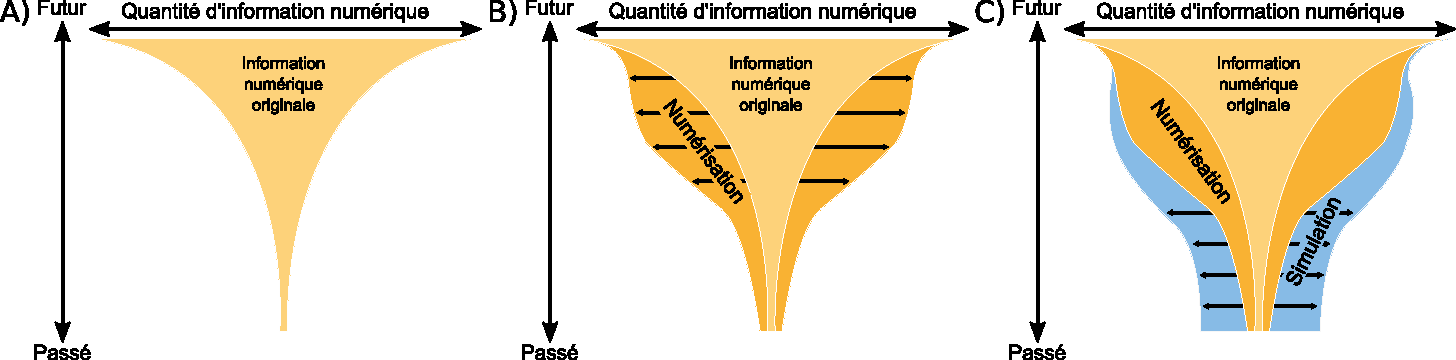
\includegraphics[width=\linewidth]{img/champignon_informationnel_kaplan.pdf}
	\caption{Le \og champignon informationnel\fg{} de \textcite{kaplan_lancement_2013}.}
	\label{fig:champignon-kaplan}
\end{figure}

L'exercice de la modélisation demande pourtant une quantité substantielle de données, et surtout que ces données soient homogènes en terme de couverture spatio-temporelle et en terme de certitude au risque que des \og effets de source\fg{} ne biaisent les résultats.
Afin d'augmenter la couverture spatio-temporelle, on a recours à des sources variées -- matérielles, écrites, voire biologiques --, par nature hétérogènes.

Les éléments empiriques ne peuvent dès lors reposer que sur une connaissance large et diversifiée des périodes et régions étudées.
Cette connaissance, que l'on peut qualifier d'experte, est l'apanage des \og thématiciens\fg{} du projet.
Le modélisateur, qui ne peut imaginer acquérir l'ensemble des connaissances expertes des thématiciens, doit accepter de leur faire entièrement confiance quant aux éléments empiriques mobilisés dans le modèle et par les biais desquels les modèles seront ensuite évalués.

Cela mène à une double implication en matière d'illégitimité.
Pour le modélisateur, cela implique qu'il sera toujours nécessaire de s'en remettre à la connaissance experte d'une personne (ou d'un groupe), sans possibilité d'ailleurs d'enrichir ces connaissances de son côté : mobiliser une référence scientifique dans une thématique de recherche inconnue ou distante, c'est risquer de citer des travaux non reconnus par la communauté, dépassés, ou encore anecdotiques.
Dans cette thèse, les tentations de référencer certains éléments empiriques en menant des recherches bibliographiques ont été nombreuses, mais sans vision d'ensemble de l'historiographie de ces sujets, cela n'ajouterait en fait aucun gage de scientificité.

Pour le thématicien, cela implique d'être en permanence \og malmené\fg{} par un modélisateur en recherche de connaissances plus précises et exhaustives.
Pierre \textsc{Garmy} le résume ainsi à propos de son expérience en tant que thématicien dans le projet TransMonDyn :
\begin{quotation}
\noindent \og La collaboration interdisciplinaire entre thématiciens et modélisateurs suppose le dépassement de deux contradictions : exhaustivité tendancielle \textit{vs} parcimonie recherchée d’une part et complexité \textit{vs} schématisation ou stylisation d’autre part.

\noindent Il existe un véritable paradoxe entre l’incomplétude de fait des données -- que les spécialistes disciplinaires cherchent à combler progressivement par l’enrichissement continu des corpus au moyen de recherches appropriées, rentabilisées par la définition de problématiques préalables aussi pointues que possible -- et l’attente des interlocuteurs modélisateurs qui veulent tout savoir et se bercent souvent d’illusions sur l’état de l’art réel dans chaque champ de connaissances. \fg{} \\
\mbox{}~ \textsc{Garmy} P., \og Annexe 1 - Retour sur expérience d’un “thématicien” \fg{}, in \textcite[476]{ouriachi_lelaboration_2017}  	  
\end{quotation}

\subsection{Un contexte fortement interdisciplinaire}

L'interdisciplinarité est le dernier élément marquant du contexte dans lequel ce travail de thèse a été initié, et qui l'aura influencé et incliné jusqu'à son terme.
Celle-ci est au cœur d'un projet tel que TransMonDyn, où collaboraient des géographes, archéologues et historiens, informaticiens et géomaticiens, épistémologues, linguistes, mathématiciens\ldots{}
Une expérience précédente, Archeomedes \autocite{durand1998archaeomedes}, avait déjà posé les bases d'une certaine interdisciplinarité entre géographes et archéologues\footnote{
	On se réfère ici aux chercheurs en géographie humaine et/ou urbaine.
	En géomorphologie, géophysique et géographie environnementale, les collaborations entre géographes et archéologues, sur des questions techniques notamment, sont plus fréquentes et anciennes.
}, et plusieurs de ses membres historiques se sont donc retrouvés dans TansMonDyn.
Ce \og noyau dur\fg{} a constitué le pôle auxquels se sont agrégés d'autres chercheurs des disciplines mentionnées, et y compris, en archéologie, des chercheurs qui avaient marqué une franche opposition aux approches très empruntes de systèmes complexes d'Archéomedes \autocite[voir][par exemple]{ferdiere_modelisation_2000}.

Au regard des enjeux du projet TransMonDyn, l'interdisciplinarité qui le caractérise s'exprime et contraint son ambition au moins de deux manières, que l'on pourrait rapporter aux domaines thématiques et méthodologiques.

\paragraph{Interdisciplinarité et thématique.} 
En premier lieu, et au plus évident, une forte interdisciplinarité implique des points de vue thématiques très différents.
Il me semble que ceux-ci sont fortement liés aux sources manipulées.
Les données statistiques et issues d'enquêtes contemporaines de la géographie urbaine, les textes et la littérature grise historique ou les traces et matériaux archéologiques, tous ces éléments sur lesquels les disciplines se constituent influencent fortement la manière de considérer un thème commun, comme par exemple celui de l'étude d'un système de villes donné.
Les géographes en analyseront les interactions et populations au moyen de données de recensement ou d'analyses des acteurs territoriaux.
Les historiens se référeront aux sources historiques, le plus souvent issues des élites ou structures dominantes, qui donneront sans doute des liens politiques ou religieux très détaillés entre les villes.
Les archéologues chercheront dans les traces matérielles des points communs en terme de nature de construction, de répartitions spatiales à l'échelle des lieux de fouilles etc.
Ces descriptifs, certes caricaturaux, montrent bien que pour une thématique commune, la disponibilité et couverture spatio-temporelle des sources privilégiés par telle ou telle discipline orientera nécessairement l'approche.

Ces sources et perspectives différentes orientent aussi fortement les ontologies et lexiques utilisés.
On a donné l'exemple des villes, mais au délà, chaque discipline use de son propre jargon et y attribue des concepts spécifiques.
Un des défis de l'interdisciplinarité, du point de vue des thématiques, est alors de parvenir à expliciter, en usant d'une formalisme (définitions, ontologies\ldots) commun de manière à ne pas laisser de place à l'implicite disciplinaire.

Découle de cette différence de vocabulaire et de sources considérées une approche nécessairement variée en terme de recherche d'explication des processus observés.
Dans cette thèse, il me semble que c'est assez visible, on a essayé de concilier les explications en intégrant l'ensemble des éléments constitutifs du système modélisé qui semblaient, pour l'un ou l'autre des thématiciens, pouvoir apporter une part d'explication.
Il fallait ainsi concilier la vision d'une géographe modélisatrice qui cherchait à expliquer la polarisation aux moyens d'attractions différenciées, la vision d'une archéologue pour qui les effets de lignages seigneuriaux et la territorialisation due aux paroisses permettaient de comprendre cette même polarisation et fixation, ou encore un historien pour qui les communautés rurales/agraires/paysannes émergentes étaient un facteur indispensable de la fixation de l'habitat rural.

Ce dernier point est aussi l'occasion d'estomper une différenciation, forte dans TransMonDyn, entre \og thématiciens\fg{}, porteurs de connaissance experte vis-à-vis des processus étudiés, et \og modélisateurs\fg{}, porteurs eux aussi d'une connaissance experte vis-à-vis de la manière de modéliser ces processus.
A mon sens, l'un des accomplissements de ce projet est aussi d'avoir montré que la frontière entre ces \og rôles\fg{} est fine, et extrêmement dépendante d'un positionnement particulier dans le cadre d'un projet particulier.
Au delà du poncif qui reviendrait à dire que chacun est tour à tour modélisateur ou thématicien selon son interlocuteur, il me semble ainsi pouvoir retirer de l'expérience TransMonDyn que pour modéliser en interdisciplinarité, chacun doit en même temps adopter ces deux postures, devenant un \og modélicien\fg{} selon les termes d'Arnaud \textsc{Banos} :
\begin{quotation}
	\noindent \og Sous le néologisme “Modélicien”, je désignais un type d’interaction très différent, qui avait amené Robin Cura et Cécile Tannier, tous deux géographes et modélisateurs, à s’investir avec une telle intensité et une telle profondeur dans la problématique historique de leur groupe de travail qu’ils en étaient progressivement venus à s’exprimer comme s’ils avaient été eux-mêmes longuement formés à cette discipline (cf. chapitre 11).
	L’évolution était tellement flagrante et systématiquement soulignée par les collègues historiens eux-mêmes que j’en suis même venu à émettre la possibilité d’un syndrome de TransMonDyn (en référence bien sûr au syndrome de Stockholm), défini de la manière suivante :
	“phénomène psychologique selon lequel des modélisateurs partageant longtemps la vie des thématiciens développent une empathie, voire une sympathie, ou une contagion émotionnelle avec ces derniers, devenant ainsi des modéliciens”.
	\fg{} \\
	\mbox{}~ \textsc{Banos} A., \og Annexe 3 - Petite typologie “empirique” des modélisateurs \fg{}, in \textcite[484]{ouriachi_lelaboration_2017}
\end{quotation}

\paragraph{Interdisciplinarité et méthodologie.}
Au délà des difficultés thématiques qu'elle implique, une interdisciplinarité large a aussi des retentissements en termes méthodologiques, très visibles dans le projet TransMonDyn.
La présence de géographes-modélisateurs, de géomaticiens, d'informaticiens, de mathématiciens ou encore de philosophes dans un projet résulte nécessairement dans des approches diversifées en matière de modélisation.
Le mathématicien favorisera en effet des formalismes mathématiques tels que les systèmes dynamiques ou la théorie des jeux, les philosophes préfèreront une modélisation ontologique des processus à l'oeuvre, le géographe préfèrera une entrée spatiale, potentiellement statistique par exemple autour de modèles gravitaires, et l'informaticien usera de ses habitudes en modélisation à base d'agents, proches de la programmation à base d'objets communicants.

Le panorama des approches de modélisation mobilisées dans les transitions de TransMonDyn illustre cette diversité de pratiques : on y retrouve beaucoup de modèles à base d'agents, mais aussi des modèles basés sur la théorie des jeux, ou encore un modèle conceptuel basé sur une ontologie dynamique \autocite{favory_transition_2018}.
En considérant l'historique des approches de modélisation du projet, on pourrait de plus y ajouter des modèles graphiques, sagittaux ou chorématiques.
Ces approches ont en commun une vision systémique des processus, mais les modalités de leurs mises en place s'effectuent selon des langages (informatiques ou formels) et des paradigmes (mathématiques, statistiques ou informatiques) très différents.

Au sein même des modèles implémentés au travers de systèmes multi-agents, l'hétérogénéité est forte : entre un modèle KISS\footnote{
Caractérisés ainsi par \textcite[110]{amblard_evaluation_2006} : 
\og Un premier courant, qui est une application directe du rasoir d'Occam, aussi appelé « principe de parcimonie », le mouvement KISS (Keep It Simple, Stupid !) recommande de construire des modèles qui soient analysables par la suite, suffisamment simples pour être disséqués par un humain qui observe les simulations attentivement \textelp{}.
Le positionnement de ce courant peut se résumer ainsi : rien ne sert de concevoir des modèles dont on ne pourrait étudier sérieusement les propriétés et oublier ainsi la validation interne, définie comme l'existence des bonnes propriétés du modèle dans le cadre formel de ce dernier
\fg{}.
}, un modèle descriptif, voir un modèle comportemental individu-centré, les paradigmes mobilisés sont entièrement différents et surtout ont des implications en matière de conception et d'évaluation diamétralement opposées.
Du point de vue méthodologique, l'interdisciplinarité dans la conception de modèles requiert, comme pour les aspects thématiques, une forte explicitation des concepts et méthodes employés afin que l'ensemble des parties prenantes soient d'une part satisfaits des modèles produits, et d'autre part en capacité de comprendre les hypothèses et biais intrinsèques qui découlent du choix du type de modélisation.

\bigskip
\paragraph[Conclusion intermédiaire]{}
Le contexte dans lequel cette thèse a été imaginée et initiée, retracé dans cette partie, permet de mieux comprendre les enjeux -- méthodologiques et thématiques -- de ce travail.
Les membres du groupe de travail de la \og transition 8\fg{} de TransMonDyn ont continué à œuvrer ensemble, même après les fins officielles (2014) et effectives (2017, à la parution de l'ouvrage collectif \og Peupler la Terre\fg{} dirigé par \textcite{sanders2018peupler}) de ce projet de recherche interdisciplinaire.
Le modèle SimFeodal, et cette thèse plus largement en constituent l'un des aboutissements.

Ma thèse, en tant que telle, n'a pourtant pas été réalisée dans le cadre officiel de l'ANR TransMonDyn.
Le présent travail de thèse a ainsi bénéficié d'un financement du LabEx DynamiTe\footnote{
Laboratoire d’Excellence \og Dynamiques Territoriales et Spatiales\fg{}, ANR-11-LABX-0046, dans le cadre du programme \og Investissements d’Avenir\fg{}.
}, proposé par le groupe de travail \og Systèmes de Peuplement sur le temps long\fg{}\footnote{
Co-dirigé par Patrice \textsc{Brun}, Marie-Vic \textsc{Ozouf-Marignier} et Lena \textsc{Sanders}.
}, dont l'obectif initial était de \og croiser les connaissances et savoir-faire de géographes, historiens, archéologues et mathématiciens pour décrire, conceptualiser et modéliser les dynamiques du peuplement sur le temps long dans leurs expressions spatiales et leurs rythmes temporels\fg{}\footnote{
Descriptif du groupe de travail : \href{http://labex-dynamite.com/fr/recherches/groupes-travail/les-systemes-de-peuplement-sur-le-temps-long/}{http://labex-dynamite.com/fr/recherches/groupes-travail/les-systemes-de-peuplement-sur-le-temps-long/}
}.
Au regard de ces objectifs, on comprendra aisément les similarités avec TransMonDyn, que ce soit en terme d'interdisciplinarité ou de démarche.

Dans les faits, ce groupe de travail \og temps long\fg{}, dans lequel je me suis inscrit tout au long de mon travail de thèse, a surtout œuvré à la résolution d'une des difficultés de l'interdisciplinarité décrite plus haut : la mise en place d'un vocabulaire commun et explicite sur les concepts et notions liés à la description et à la modélisation des systèmes de peuplement sur le temps long.
La réalisation du \og lexique spatio-temporel illustré\fg{} -- nom provisoire qui a par la suite été abandonné -- qui en résulte, intitulé \og « Les concepts-clés des systèmes de peuplement sur le temps long » (\hl{ajouter ref, voir avec Lena}), a nourri l'ensemble de cette thèse, en contribuant largement à mettre au clair les concepts employés.
À ce titre, le groupe de travail du LabEx a aussi constitué un contexte fort, en mettant en place des discussions interdisciplinaires, autour des mêmes disciplines mais avec une communauté de chercheurs et d'approches de ces disciplines très différente de celles de TransMonDyn.


\section{Quel questionnement et évolution ?}

\subsection{Sujet initial}

\subsection{Verrous}

\subsection{Nouvelles questions}

\section{Quelle position ?}

\subsection{Co-construction}

\subsection{Interface}

\subsection{Démarche exploratoire}

\section*{Conclusion}
\addcontentsline{toc}{section}{\protect\numberline{}Conclusion}